\section{Invarianter för studenters laborationsantal}

Det finns möjlighet att ha en invariant mellan hur många simultana “laboration-till-grupp”-kopplingar det finns per laboration för varje enskild student. Det rör sig mellan alternativen att forcera maximalt en koppling per laboration, att forcera till exakt en koppling per laboration samt att strunta i att ha invarianten. Det leder till mer arbete att uppehålla en striktare invariant, men det har fler fördelar.

För att göra detta avsnitt läsbart inför vi termen LabHasGroup, förkortad \emph{LHG}. \emph{LHG} är den entitet i modellen som representerar kopplingen mellan en grupp och en laboration, vilket beskrivs i sektion \ref{sec:modell-labhasgroup}. 

\subsection{Max en \emph{LHG} per laboration ($\leq 1$)}
Som en direkt konsekvens av denna invariant kan inte en student lämna in samma laboration genom flera laboration till grupp kopplingar eftersom invarianten direkt stryper kopplingsantalet till maximalt en per laboration. I praktiken jobbar aldrig en student på samma laboration via flera kopplingar samtidigt. Det är troligt att studentanvändare blir förvirrade av att de ser att de jobbar på samma laboration via olika kopplingar. Det bör alltså noteras att fördelarna är främst  ytliga, alltså att produktens webbinterface blir tydligt för studentanvändarna. Vidare ska en handledare inte av misstag behöva rätta två inlämnade laborationer kopplade till samma student.

Flera möjliga sätt finns för att enforcera invarianten, gemensamt för implementeringssätten är att de måste definera nödvändiga gruppoperationer och visa att de är riskfria, det vill säga att invarianten aldrig bryts efter operationerna har utförts. Några operationer kan tänkas vara följande:

\begin{itemize}
  \item Skapa grupp
  \item Gå med i grupp
  \item Eventuellt “starta laboration”
  \item Ta bort,  inaktivera eller frysa en laboration – dessa operationer är ekvivalenta
\end{itemize} 

Eftersom grupperna är immuterbara finns inte operationerna elevavhopp eller gruppsplittring. Invarianten syftar på antalet aktiva grupper vilket skulle betyda att operationerna: ta bort, inaktivera samt frysa en \emph{LHG} är alla ekvivalenta vad berör denna invariant.  Att starta en laboration behöver inte finnas som operation. Exempelvis är det möjligt att definiera att en gruppstart, per automatik, skapar samtliga \emph{LHG}:s. Ovanstående är alltså en minimal grund för att kunna beskriva implementationer av invarianterna.

\subsubsection{Förslag på implementering}
En operationsuppsättning kan vara att en grupp alltid skapas tom utan \emph{LHG}s, att en student bara kan gå med i grupper utan \emph{LHG}s samt att operationen “starta laboration” bara är utförbar då samtliga elever i gruppen saknar \emph{LHG}s för den laborationen. En student kan ta bort sin \emph{LHG}. Notera att denna operation måste finnas för att samma student någonsin ska kunna starta en ny \emph{LHG} till samma laboration. Denna operationsuppsättning utgör en implementering och ansågs av vår grupp till att vara den enklast genomförbara.


\begin{proof}[Bevis av korrekthet]
  Vi har medvetet försökt minimera antalet operationer som påverkar antalet kopplingarern student har till en given laboration. Att skapa en grupp påverkar ej \emph{LHG}-antalet. Att gå med i en grupp har begränsats till att bara fungera för grupper utan påbörjade laborationer, därav påverkas ej invarianten av påhopp heller. Att ta bort en \emph{LHG} innebär en minskning vilket aldrig kan bryta mot en “mindre-än”-olikhet. Den enda operationen som ökar antalet \emph{LHG}s är att “påbörja laborationen”, men den har definierats att bara vara utförbar då invarianten inte bryts. \qedhere
\end{proof}

\subsubsection{Användarperspektiv}
Operationerna som krävs för att byta \emph{LHG} från en grupp till en annan är: skapa den nya gruppen, bjud in dina nya laborationskamrater som måste därefter ta bort samtliga \emph{LHG}:s hos sina nuvarande grupper för att sedan kunna skapa den nya \emph{LHG}:en i den nya gruppen, även ens tidigare laborationskamrater måste troligen göra detta. Stegen är förklarade i  figurserie \ref{fig:slack_series}.

\begin{figure}
  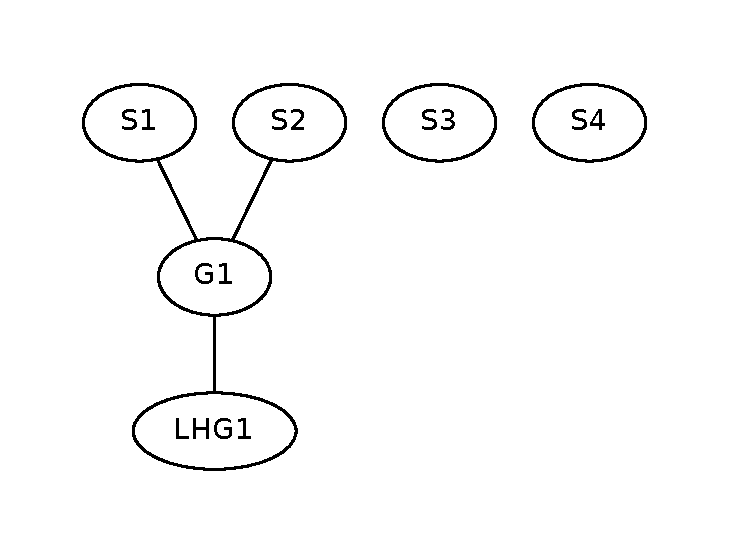
\includegraphics[width=7.0cm]{fig/labgroup/slack_add_1.pdf}        
  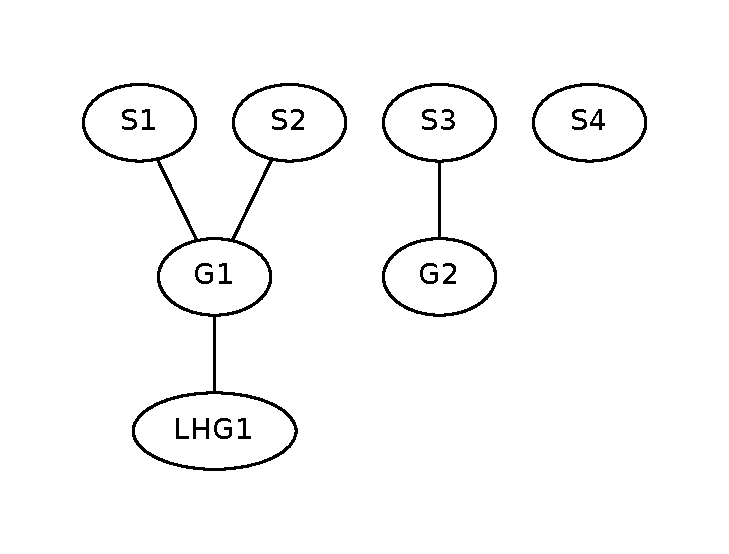
\includegraphics[width=7.0cm]{fig/labgroup/slack_add_2.pdf}        
  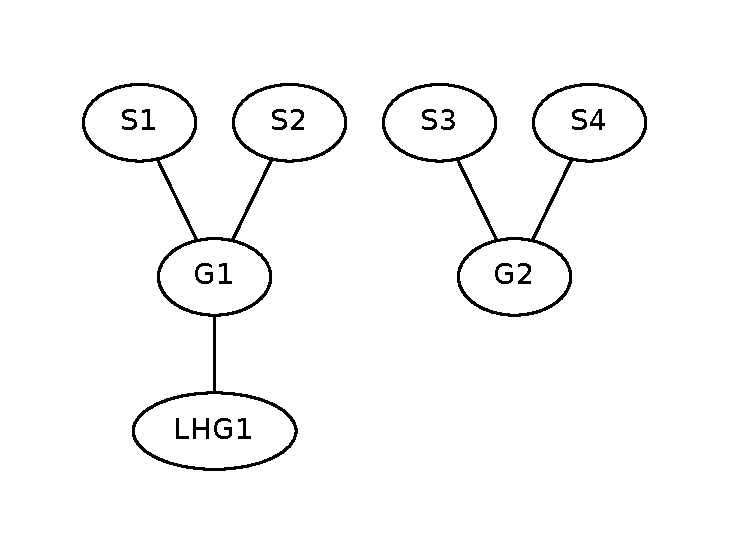
\includegraphics[width=7.0cm]{fig/labgroup/slack_add_2-5.pdf}        
  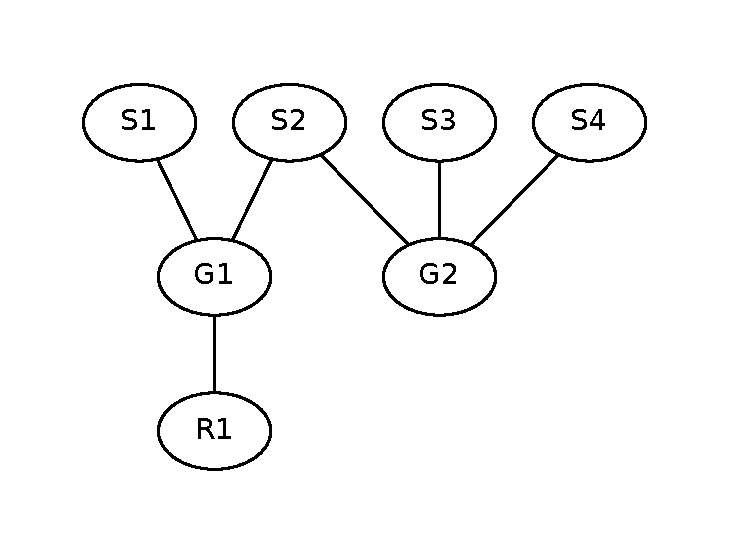
\includegraphics[width=7.0cm]{fig/labgroup/slack_add_3.pdf}        
  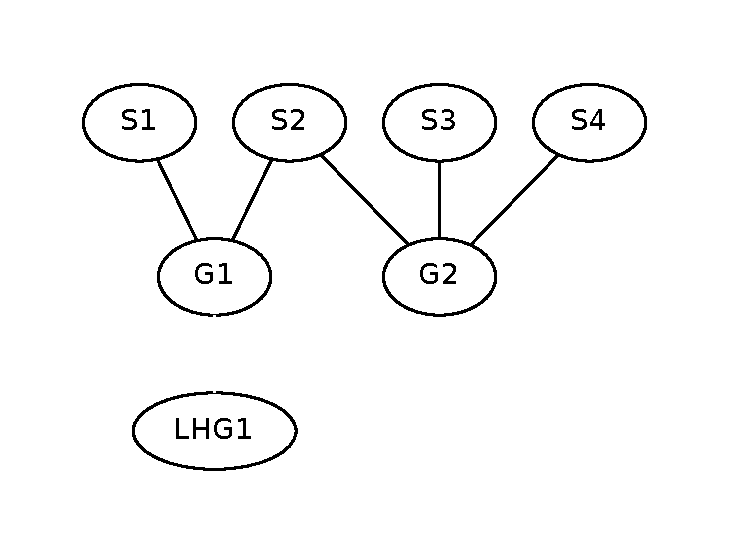
\includegraphics[width=7.0cm]{fig/labgroup/slack_add_4.pdf}        
  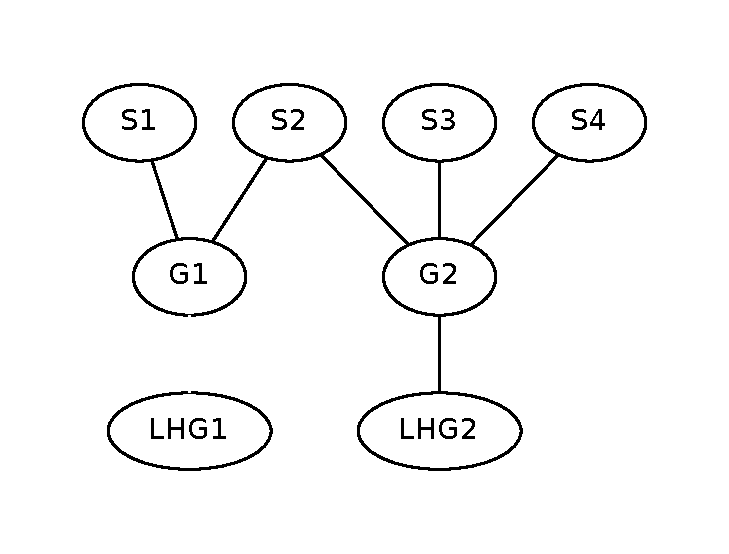
\includegraphics[width=7.0cm]{fig/labgroup/slack_add_5.pdf}        
  \caption[Serie tillstånd rörande labgrupper.]
  {Serie tillstånd rörande labgrupper. Studenterna $S2$, $S3$ och $S4$ vill
  bilda en ny laborationsgrupp tillsammans (den som blev $G2$) där de ska skapa
  en \emph{LHG}. Notera hur student $S2$ måste ta bort sin förra \emph{LHG} innan någon elev
  kan lägga till en \emph{LHG} i den nya gruppen. Mellan varje figur krävs att någon
  användare gör en åtgärd i waters system.}
  \label{fig:slack_series}
  
\end{figure}

\subsection{Alltid exakt en \emph{LHG} per laboration ($= 1$)}
Den mindre strikta ($\leq 1$) invarianten ger Water möjligheten att ha ett intuitivt användargränssnitt eftersom ingen student vill se att de gör samma laboration via två olika grupper samtidigt. En striktare variant är dock önskvärd av tekniska skäl. Med en striktare variant behövs till exempel inte hantering av fall då en \emph{LHG} inte finns, eftersom att den alltid finns. Detta öppnar även upp för att förenkla våra databasförfrågningar, vi kan till exempel få reda på alla laborationer för en student i en kurs genom att “gå” via kopplingarna, eftersom vi har en 1-till-1–relation mellan “laboration-till-grupp”-koppling och laboration per student.

En operationsuppsättning för denna invariant måste även definiera initialtillståndet eftersom det går inte längre att ha studenter utan \emph{LHG}:s vid kursstart. Operationerna som måste beaktas för denna invariant är fler eftersom tillägg av student eller laboration både är icketriviala. Ifall en student läggs till i en kurs så måste den “direkt” få sina \emph{LHG}:s. Laborationstillägg måste även se till att varje student får en \emph{LHG} för den nyligen skapade laborationen. En operation som inte längre kan finnas är att manuellt ta bort en \emph{LHG} för då skulle invarianten brytas direkt.

\subsubsection{Förslag på implementering}
Invarianten kan  framtvingas genom följande initialtillstånd och operationsuppsättning.

\paragraph{Initialtillstånd}
I början är alla studenter inplacerade i en för varje student unik grupp som kallas “studentens grupp” (förkortat SG i figurerna). Varje student har en sådan grupp som innehåller en \emph{LHG} till alla laborationer som finns registrerade i kursen. Se figur \ref{fig:strict-initstate}.

\begin{figure}
  \centering
  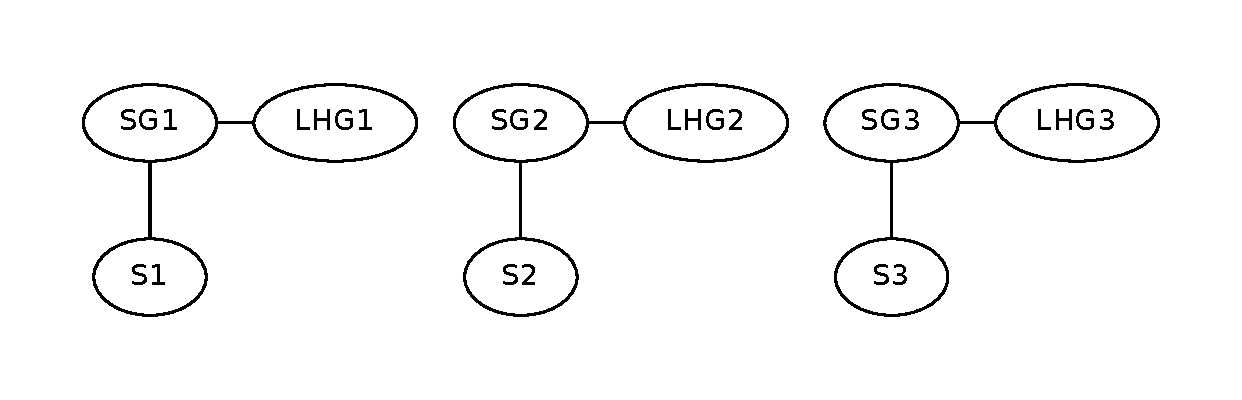
\includegraphics[width=8.0cm]{fig/labgroup/strict_initstate.pdf}
  \caption{Illustration av initialtillståndet i en kurs med 3 studenter}\label{fig:strict-initstate}
\end{figure}

\paragraph{Operationer}
I detta förslag behandlas operationerna “skapa en grupp” och “lägg till en student i gruppen” på samma sätt som i förslaget för den mindre strika invarianten. Att skapa en ny \emph{LHG} kommer inte ha kräva några förhandsvillkor, studenten behöver alltså inte längre manuellt se till så att \emph{LHG}:en sätts in genom att ta bort sina egna kopplingar i sina tidigare grupper, istället tar Water bort alla kopplingar som “är i vägen”. Operationen sker mer specifikt på följande sätt:
\begin{enumerate}
  \item För alla medlemmar i gruppen där \emph{LHG}:en ska läggas till ska
    deras \emph{LHG} för den laborationen tas bort, notera att de alltid har
    exakt en sådan på grund av invarianten.
  \item Lägg till \emph{LHG}:en, nu skall invarianten stämma för gruppmedlemmarna.
  \item Borttagningarna i första steget kan ha påverkan på studenter utanför
  den aktiva studentens laborationsgrupp. För de påverkade studenterna lägger
  vi till en \emph{LHG} i  deras egna laborationsgrupp (studentens laborationsgrupp).
  Dessa påverkade studenter kallas för “laborationskamraternas
  laborationskamrater”.

\end{enumerate}

Notera att ovanstånde deloperationer sker atomärt, alltså ingenting sker mellan stegen, detta eftersom invarianten blir bruten mellan deloperationerna.

Då en student läggs till en kurs skapas en \emph{LHG} för varje laboration som placeras i studentens grupp. Då en ny laboration skapas för en kurs så kommer varje student få en \emph{LHG} för den laborationen insatt i sin egna grupp.

\begin{proof}[Bevis av korrekthet]
I initialtillståndet är invarianten uppenbarligen uppfylld, samt även efter tillägg av student eller laboration. Den enda kvarstående operationen är skapande av en \emph{LHG} vars beskrivning delats upp i 3 deloperationer. 

Låt mängden A (se figur \ref{fig:strict-proof}) vara samtliga involverade elever som påverkas av operationen, alltså studenten som aktivt lägger till \emph{LHG}:en, laborationskamraterna till den eleven samt laborationskamraternas laborationskamrater som får sin \emph{LHG} borttagen i steg 1. 

Låt mängden B vara de elever som är med i laborationsgruppen där \emph{LHG}:en skapas i steg 2, notera alltså att B$\subseteq$A, notera även att de elever som berörs i steg 3 är A$\setminus$B.

I början antags invarianten vara uppfylld, efter steg 1 så har studenterna i A ingen \emph{LHG}, efter steg 2 har eleverna i B en ny \emph{LHG}, endast A$\setminus$B saknar var sin \emph{LHG} nu, vilket steg 3 åtgärdar. \qedhere
\end{proof}
 
\begin{figure}
  \centering
  \begin{subfigure}[b]{0.5\textwidth}
    \centering
    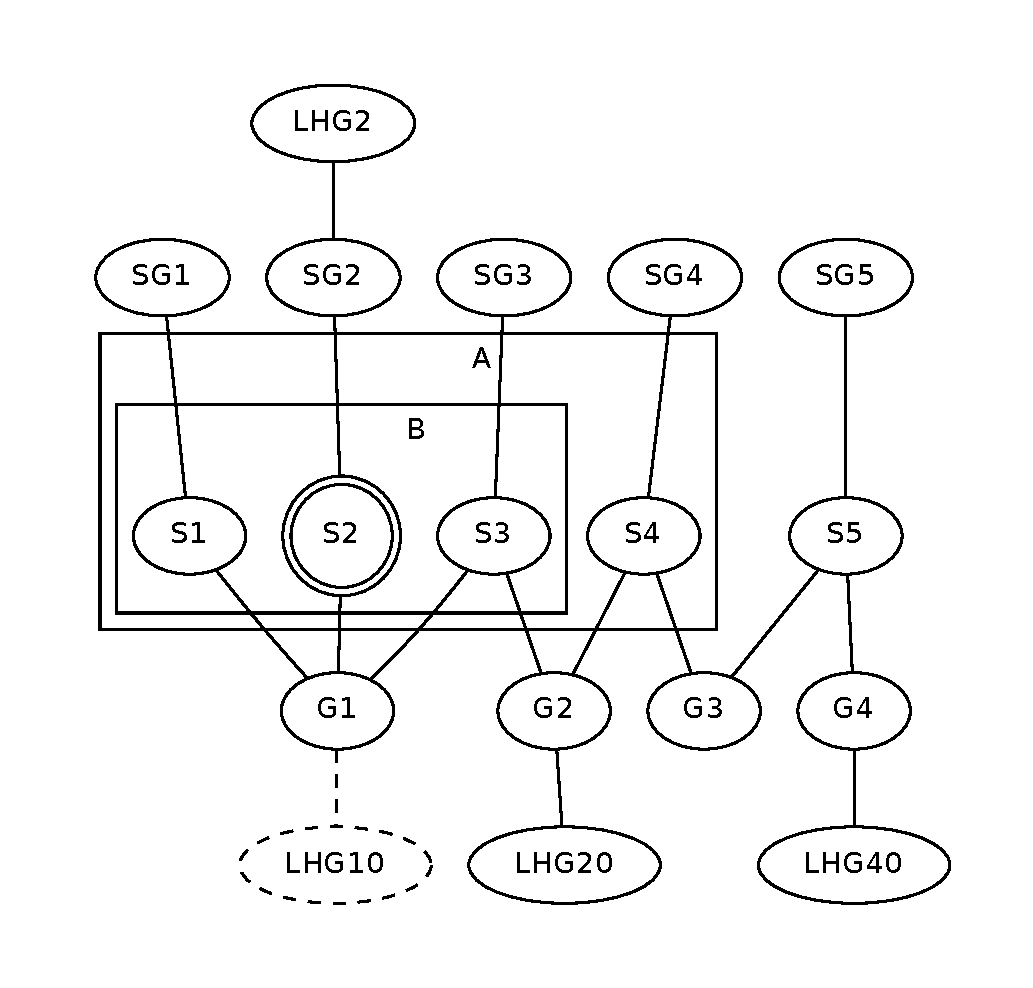
\includegraphics[width=8.0cm]{fig/labgroup/strict_proof.pdf}
    \caption{Situation när $S2$ ska lägga till $LHG10$}
    \label{fig:strict-proof}
  \end{subfigure}%
        ~ %add desired spacing between images, e. g. ~, \quad, \qquad etc. 
          %(or a blank line to force the subfigure onto a new line)
  \begin{subfigure}[b]{0.5\textwidth}
    \centering
    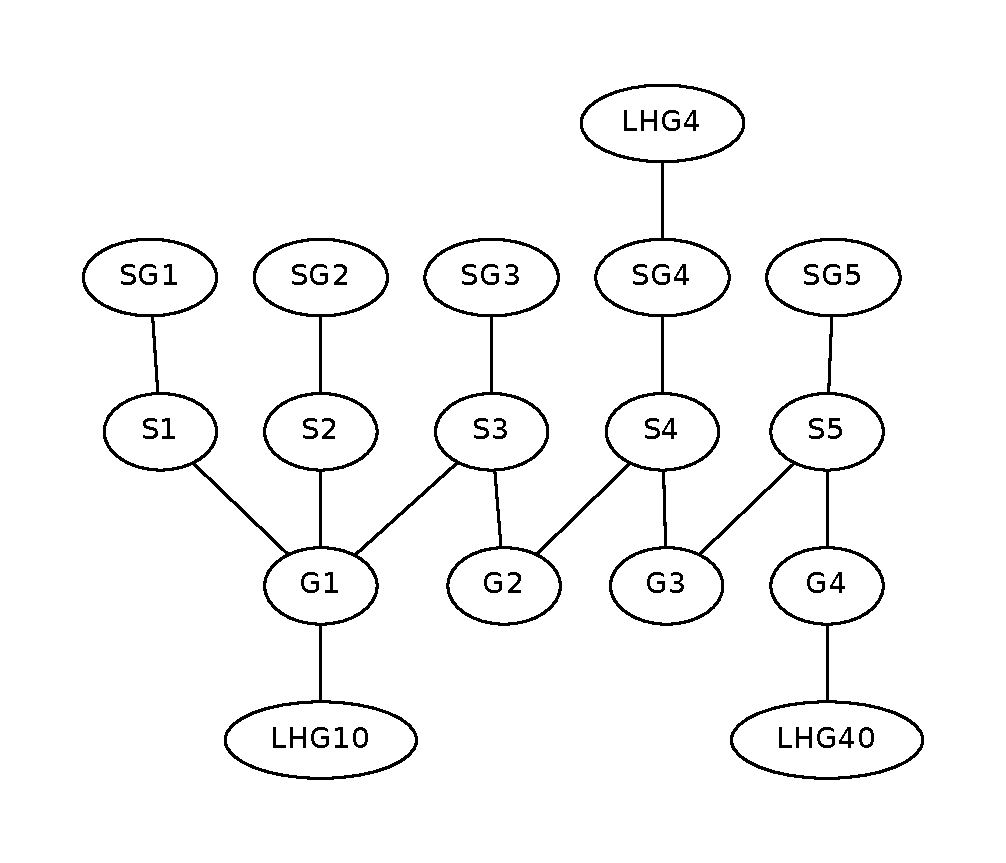
\includegraphics[width=8.0cm]{fig/labgroup/strict_proof_continue.pdf}
    \caption{Situation efter $LHG10$ lagts till}
    \label{fig:strict-proof-continue}
  \end{subfigure}
  \caption{Före och efter \emph{LHG}-tillägg (strikt invariant)}\label{fig:animals}
\end{figure}

\subsubsection{Användarperspektiv}
Det ovanstående sättet att skapa en ny \emph{LHG} innebär att även laborationskamraternas laborationskamrater påverkas av den aktiva studentens operation (se figur \ref{fig:strict-proof-continue}). Detta är givetvis inte bra för de utsatta studenterna. Att samtliga studenter har en egen laborationsgrupp kan vara förvirrande för användare som ser att de redan är medlemmar i en laborationsgrupp som är låst och redan har påbörjat sina laborationer. I gengäld kräver operationen färre steg för en student att påbörja en laboration med en annan laborationsgrupp.

\subsection{Ingen invariant}
Naturligtvis går det att strunta i att forcera någon invariant. Det blir minimalt med jobb och ingenting behöver bevisas. Nackdelen är att det lätt blir förvirrande för användaren att ha flera aktiva laborationer samtidigt. Vidare krävs fler användaroperationer för att lokalisera sin \emph{LHG} då användaren inte bara behöver specifiera laboration utan även laborationsgrupp.

\begin{flushright}
  
  \textbf{Beslut}
  
  Vi valde att implementera ($\leq 1$) invarianten. Vi satte hög prestige i ett användargränssnitt där användare direkt kan klicka på deras laboration utan att först välja laborationsgrupp.
\end{flushright}
